\documentclass[letter]{article}

\usepackage[dvipsnames]{xcolor}
\usepackage[T1]{fontenc}
\usepackage[utf8]{inputenc}
\usepackage{lmodern}

\usepackage[english]{babel}
\usepackage{csquotes}
\usepackage{multirow}

\usepackage{graphicx}
\graphicspath{ {./images/} }

\usepackage[margin=0.5in]{geometry}

\usepackage[notes,backend=biber]{biblatex-chicago}
\bibliography{sample}

\begin{document}
\title{Unsupervised Learning - CS 4641}
\author{Omar Shaikh}
\maketitle

\begin{abstract}
    In this report, I cover two fundamental unsupervised machine learning algorithms: K-means and Gaussian Mixture Models. To do this, I select two different data-sets -- images of histopathologic-cancer tumors and the classic Iris Flower Dataset. First, I introduce each dataset and our unsupervised classification problem; then, I run the clustering algorithms on the datasets and describe my results, both before and after running dimensionality reduction algorithms (ICA, PCA, Random Projections, Autoencoder). 
    
    The next section involves neural network analysis on only the Iris dataset. First, I rerun my neural network learner on only the dimension reduced datasets and discuss my results. Then, I treat the clustering algorithms as dimensionality reduction algorithms, running my neural network learner on this newly projected data. In the comparative analysis section, I test each algorithm on the withheld testing data, showcasing the strengths and weaknesses of each while answering some questions.
\end{abstract}

\section{Datasets \& Learning Problems}
\subsection{PCam Dataset \& Classification}

The first dataset I used (same as assignment \#1) is the CAMELYON dataset, collected by Department of Pathology of the Radboud University Medical Center (Radboudumc) in Nijmegen, The Netherlands \autocite{doi:10.1093/gigascience/giy065}. I found this dataset after searching for labelled cancer images datasets.

The dataset has binary labels: either the cells have metastasized (1 label), or they have not (0 label). For the sake of speed, I chose to undersample this dataset such that N=88010, instead of N=220025. The undersampled dataset has a 60-40 split. See figure 1 for a breakdown of the undersampled dataset. Finally, why this dataset? My family has an unfortunate genetic history with cancer, so a related project was generally of interest.

\subsubsection{General Feature Engineering}
Although images provided were a 96x96 slide, only the center 32x32 contained tumor tissue. For classifiers used in this report, I cropped the images and converted them to black and white beforehand. I also rescaled the image pixels to have zero mean and one standard deviation. 

\begin{figure}
  \centering
  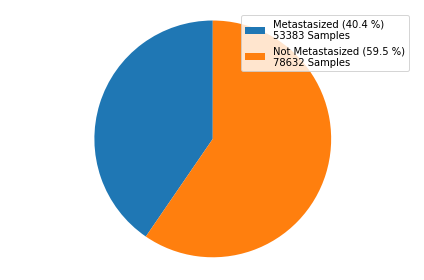
\includegraphics[width=0.4\textwidth]{images/pcamDistr.png}
  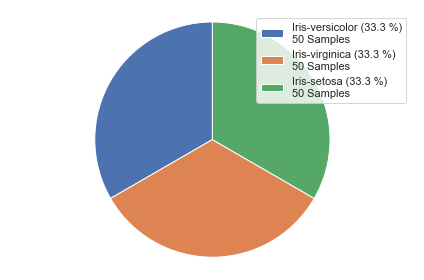
\includegraphics[width=0.4\textwidth]{images/irisDistr.png}
  \caption{Breakdown of the datasets; Undersampled PCam (left), Iris (right)}
\end{figure}

\subsection{Iris Flower Dataset}

I found the Iris flower dataset after searching for relatively low dimensional data with more than one class category. The dataset is a part of UCI's Machine Learning database\autocite{irisUCI}, and consists of 4 different features: the sepal length/width and the petal length/width.  Figure 1 highlights the breakdown of the dataset.

Finally, why this dataset? I couldn't use my old dataset from Assignment 1 because the data already underwent dimensionality reduction. I also wanted to find a dataset that could be visualized after projections so that viewing the clusters provided for a more "tangible" analysis.

\subsubsection{General Feature Engineering}
All 4 features (sepal length/width and the petal length/width) were rescaled to have 0 mean and 1 standard deviation.

\subsection{Computer Specifications}
The computer used to train and test has an i7-7700HQ (clock speeds @ 3.8 GHZ), 32 GB of RAM, and an Nvidia GTX 1070 with 8 GB of VRAM. Whenever it was possible, I used all CPU cores (n\_jobs=-1 in sci-kit). Runtimes of algorithms should be considered in context of these specifications.

\section{Part I: Clustering}
\subsection{Measures for Picking K}
To pick K, I decided to rely on two measures for evaluating the clusters.

My first measure, purity, was picked for its simplicity and is only used on PCam. Each cluster is assigned to the class which appears most frequently in the cluster. Then, we take the average of each cluster's accuracy in assigning the most frequent label. Formally: $\frac{1}{N}\sum_k \max_j\vert\omega_k \cap c_j\vert$, where $\{ \omega_1, \omega_2, \ldots, \omega_K \}$is the set of clusters and $\{ c_1,c_2,\ldots,c_J \}$ is the set of classes\autocite{Manning:2008:IIR:1394399}.

Second, I decided to use cluster V-Measure\autocite{RosenbergH07}. V-Measure works by taking the harmonic mean of two properties: cluster homogeneity and completeness. Homogeneity "is satisfied if each cluster contains only members of a single class." Completeness, on the other hand "is satisfied if all members of a given class are assigned to the same cluster." Both are bounded between 0 and 1, inclusive.

Completeness (c) and homogeneity (h) can be defined as follows: $h = 1 - \frac{H(C|K)}{H(C)}$ and $c = 1 - \frac{H(K|C)}{H(K)}$, where $H(C|K)$ is the conditional entropy of the classes given assignments and $H(C)$ is the entropy of the classes. What I found interesting is that V-measure can be interpreted using principles of information theory. Unlike purity, there's also a penalization behind picking more clusters, as seen by the following relation: $v = 2 \cdot \frac{h \cdot c}{h + c}$. As entropies increase without payoff, the harmonic mean "normalizes" the quantity, reducing the overall V-measure. The justification behind this lies on assuming that entropy generally increases as cluster size increases.

Theoretically, purity can be maximized by picking as many clusters as there are samples; however, its transparency and simplicity are benefits. For both measures, no assumption is made on the cluster structure. Thus, they can be used to compare clustering algorithms like K-means and EM without bias.

Finally, to pick the K-value itself based on the measure, I rely on the elbow method -- picking a K where K + 1 won't improve our measures (Figure 2 and 3 for PCam, Figure 7 for Iris) by a significant amount\autocite{Thorndike1953}.

\subsection{Results and Analysis}
My search space was from $1 \leq k \leq 10$ for PCam and Iris. Table 1 highlights the best values of k given our datasets and algorithms.

\subsubsection{PCam}
For GMM, the optimum value of clusters for our untouched (un-"dimensionality reduced") dataset appears to be K = 5; with this cluster number, we maximize homogeneity and purity relative to eachother. Refer to the right side of Figure 2 and 3. For K-means, the best number of clusters is 3, again using the elbow method. Note that the autoencoder, PCA, and the untouched dataset return similar results -- this will be addressed later.

I tried visualizing the clusters using T-SNE, but because of the high dimensionality of the data, the projections looked worse than the actual classification accuracy metric. However, I suspect that K-means forms very basic clusters as the purity score mirrors the distribution of classes in the dataset. I also suspect that the Euclidean distance is the damning factor behind the low performance. The following reasoning also comes from Assignment \#1's KNN classifier:
\begin{quote}
  The use distance metrics on raw pixel values is not adequate since the distances correlate more strongly with backgrounds and color distributions of images than with their semantic content.\autocite{Stanford-Img} 
\end{quote}

Being a hard clustering algorithm also limits K-means from exploiting the generally normal distribution of image pixels. Comparatively, GMMs use Gaussian Models to pick out the underlying image pixel distributions to gain an edge in clustering accuracy. This becomes apparent when we look at the individual purity scores for the GMM and K-mean clusters: $GMM=[0.90, 0.80, 0.78 , 0.61, 0.55]$, $Kmeans=[0.81, 0.61, 0.57]$. Note that these purity scores also shed light on why the number of clusters make sense. 

KMeans picks out one good cluster with a high purity score, but we see a significant drop in the other two. It finds a single distinguishing factor for the first cluster, but can't improve on the other clusters. GMM, however, improves accuracy on more sub-clusters, and reduces the proportion of clusters it does poorly on. Because K-means uses distance as a primary metric, it limits the number of clusters (and distinguishing features) that can be observed using GMMs -- this explains why the K results we observed make sense.

Note that the increased accuracy of GMM comes with a price: speed (see Figure 4).

\begin{figure}
  \centering
  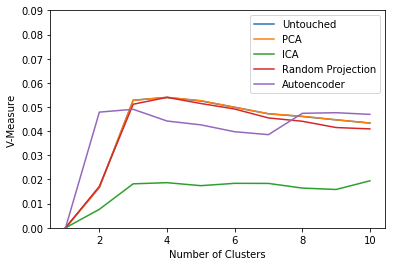
\includegraphics[width=0.4\textwidth]{images/pcamKmeansHomo.png}
  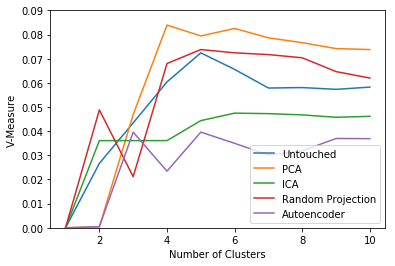
\includegraphics[width=0.4\textwidth]{images/pcamGMMHomo.png}
  \caption{V-Measure scores on PCam; KMeans (left), GMM (right)}
\end{figure}

\begin{figure}
  \centering
  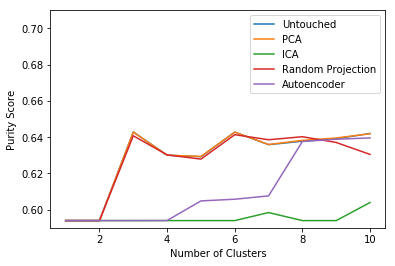
\includegraphics[width=0.4\textwidth]{images/pcamKmeansPurity.png}
  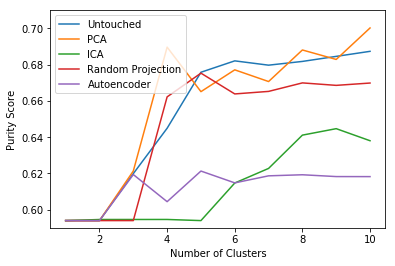
\includegraphics[width=0.4\textwidth]{images/pcamGMMPurity.png}
  \caption{Purity scores on PCam; KMeans (left), GMM (right)}
\end{figure}

\begin{figure}
  \centering
  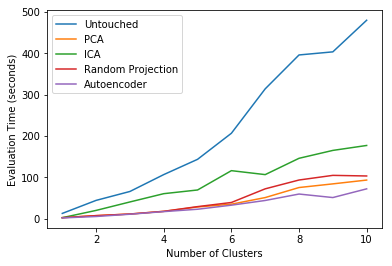
\includegraphics[width=0.4\textwidth]{images/kmeansTime.png}
  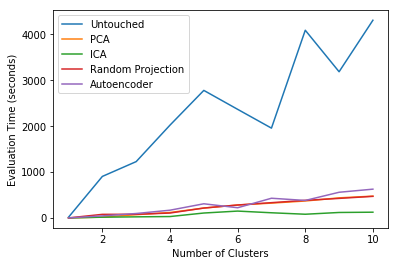
\includegraphics[width=0.4\textwidth]{images/gmmTime.png}
  \caption{Clustering Evaluation Times on PCam; KMeans (left), GMM (right)}
\end{figure}

\begin{figure}
  \centering
  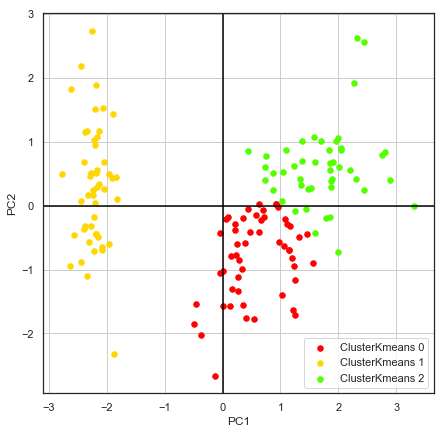
\includegraphics[width=0.4\textwidth]{images/kmeansUntouchedIris.png}
  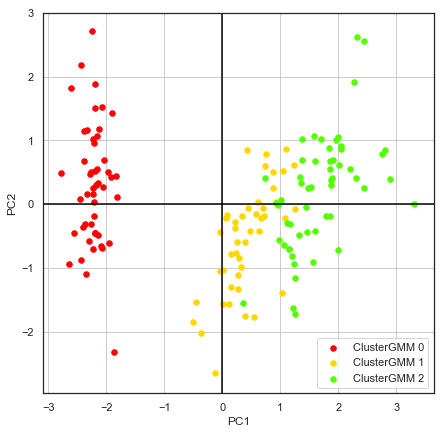
\includegraphics[width=0.4\textwidth]{images/gmmUntouchedIris.png}
  \caption{Clustering on Untouched Iris Dataset for KMeans (left); GMM (right). Projected using PCA.}
\end{figure}

\begin{figure}
  \centering
  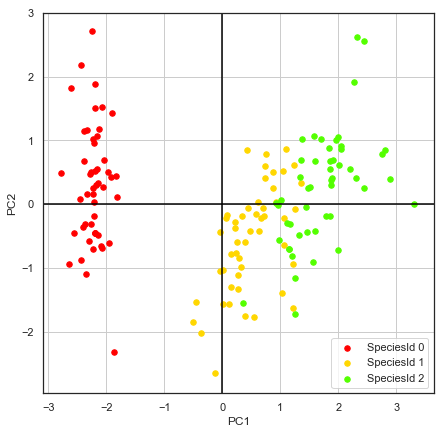
\includegraphics[width=0.24\textwidth]{images/groundTruthIris.png}
  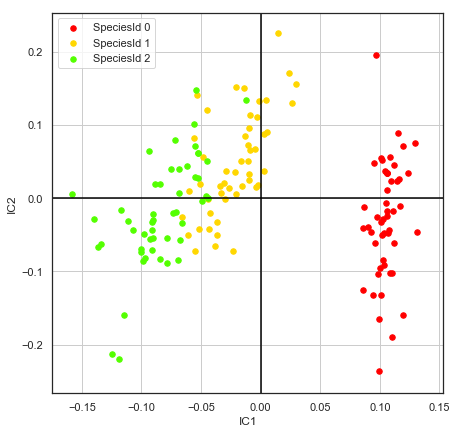
\includegraphics[width=0.24\textwidth]{images/groundTruthICA.png}
  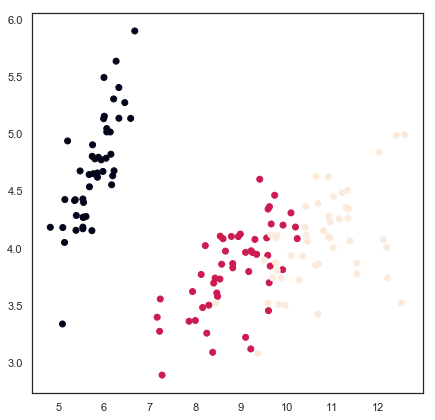
\includegraphics[width=0.24\textwidth]{images/groundTruthAutoencoder.png}
  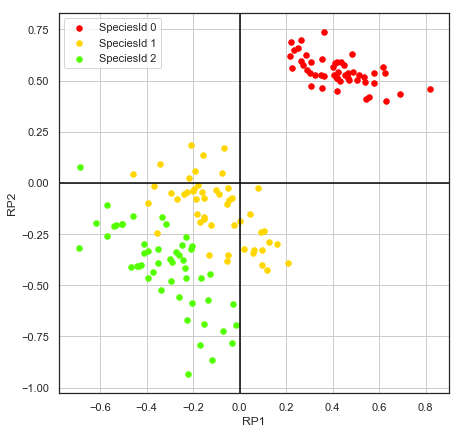
\includegraphics[width=0.24\textwidth]{images/groundTruthRP.png}
  \caption{Ground Truth on Projected Iris Untouched Dataset.}
  Left to Right: PCA (1st); ICA (2nd); Autoencoder (3rd); RP (4th)
\end{figure}

\begin{figure}
  \centering
  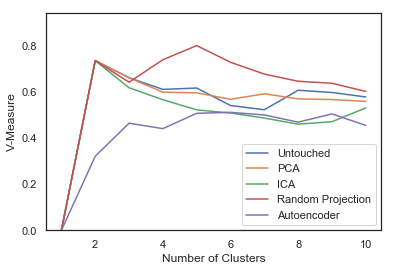
\includegraphics[width=0.4\textwidth]{images/irisKmeansVmeasure.png}
  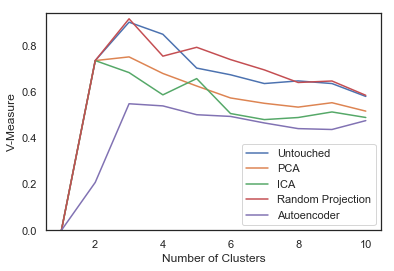
\includegraphics[width=0.4\textwidth]{images/irisGmmVmeasure.png}
  \caption{V-Measure scores on Iris; KMeans (left), GMM (right)}
\end{figure}

\begin{figure}
  \centering
  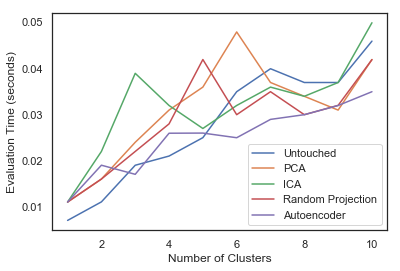
\includegraphics[width=0.4\textwidth]{images/kmeansIrisTime.png}
  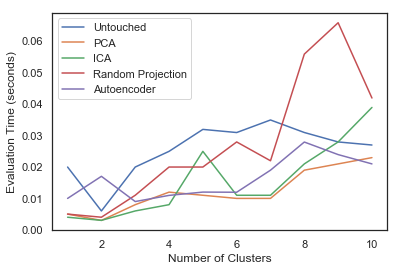
\includegraphics[width=0.4\textwidth]{images/gmmIrisTime.png}
  \caption{Clustering Evaluation Times on Iris; KMeans (left), GMM (right)}
\end{figure}

\subsubsection{Iris}
For both K-means and GMM, the optimum number of clusters is 3, something I expected given that the number of classes was 3. However, GMM performs far better than K-means for all values of K. I also expected this because several natural phenomena can be explained using a gaussian/normal model.

Although PCA is covered more thoroughly a following section, Figure 5 projects our dataset onto two dimensions (using 2 principal components) and highlights cluster labeling between between K-means and GMM run on the original dataset. Notice why GMM has an advantage; while K-means refuses to do soft margin clustering, the EM algorithm correctly assigns labels to the trickier samples. The ground truth labels can be seen in Figure 6 (left). 

Unlike PCam, we're not penalized by reduced speed when we use GMM (Figure 8), probably because our dataset size is relatively small.

\subsection{Improving Performance}
In the case of PCam, as we bumped our cluster sizes, our V-measure kept increasing. Perhaps there's another elbow beyond our search space that I hadn't yet discovered. Also, keeping color channels in PCam may have bumped our metrics. For Iris, I would experiment with other clustering performance metrics. Sometimes, our metrics point at two clusters as the optimal number, which is nonsensical, since we have 3 classes. V-Measure appears to prefer getting an entire class wrong than taking a risk by creating another cluster.

\begin{table}
  \centering
  \begin{tabular}{cc|c|c|c|}
  \cline{3-5}
   &  & \multicolumn{2}{c|}{PCam} & Iris \\ \cline{3-5} 
   &  & Purity & V-Measure & V-Measure \\ \hline
  \multicolumn{1}{|c|}{\multirow{2}{*}{Untouched}} & K-Means & .64 (k=3) & .053 (k=3) & .73 (k=2) \\ \cline{2-5} 
  \multicolumn{1}{|c|}{} & GMM & .68 (k=5) & .073 (k=5) & .90 (k=3) \\ \hline
  \multicolumn{1}{|c|}{\multirow{2}{*}{PCA}} & K-Means & .64 (k=3) & .053 (k=3) & .73 (k=2) \\ \cline{2-5} 
  \multicolumn{1}{|c|}{} & GMM & \textbf{.68 (k=4)} & \textbf{.084 (k=4)} & .73 (k=3) \\ \hline
  \multicolumn{1}{|c|}{\multirow{2}{*}{ICA}} & K-Means & .60 (k=7) & .018 (k=7) & .73 (k=2) \\ \cline{2-5} 
  \multicolumn{1}{|c|}{} & GMM & .64 (k=9) & .046 (k=9) & .73 (k=2) \\ \hline
  \multicolumn{1}{|c|}{\multirow{2}{*}{RP}} & K-Means & .64 (k=3) & .051 (k=3) & .79 (k=5) \\ \cline{2-5} 
  \multicolumn{1}{|c|}{} & GMM & .68 (k=4) & .074 (k=4) & \textbf{.91 (k=3)} \\ \hline
  \multicolumn{1}{|c|}{\multirow{2}{*}{Autoencoder}} & K-Means & .64 (k=9) & .048 (k=9) & .50 (k=4) \\ \cline{2-5} 
  \multicolumn{1}{|c|}{} & GMM & .62 (k=3) & .040 (k=3) & .51 (k=6) \\ \hline
  \end{tabular}
  \caption{Purity and V-Measure results for optimal values of K on PCam and Iris datasets}
\end{table}

\begin{table}
  \centering
  \begin{tabular}{l|l|l|l|l|}
  \cline{2-5}
                                 & PCA                        & ICA                        & Autoencoder              & RP                        \\ \hline
  \multicolumn{1}{|c|}{MSE Loss} & \multicolumn{1}{c|}{.1574} & \multicolumn{1}{c|}{.1569} & \multicolumn{1}{c|}{.64} & \multicolumn{1}{c|}{5.56} \\ \hline
  \multicolumn{1}{|c|}{Fit Time (min)} &\multicolumn{1}{c|}{.12}&\multicolumn{1}{c|}{1.22}&\multicolumn{1}{c|}{16.72}&\multicolumn{1}{c|}{.39} \\ \hline
  \end{tabular}
  \caption{MSE loss and Fit Times (mins) for Dimensionality Reduction on PCam}
\end{table}

\begin{table}
  \centering
  \begin{tabular}{l|l|l|l|l|}
  \cline{2-5}
                                 & PCA                        & ICA                        & Autoencoder              & RP                        \\ \hline
  \multicolumn{1}{|c|}{MSE Loss} & \multicolumn{1}{c|}{.042} & \multicolumn{1}{c|}{.042} & \multicolumn{1}{c|}{.54} & \multicolumn{1}{c|}{.015} \\ \hline
  \multicolumn{1}{|c|}{Fit Time (sec)} &\multicolumn{1}{c|}{.002}&\multicolumn{1}{c|}{.003}&\multicolumn{1}{c|}{35.3}&\multicolumn{1}{c|}{3.5} \\ \hline
  \end{tabular}
  \caption{MSE loss and Fit Times (sec) for Dimensionality Reduction on Iris}
\end{table}

\begin{figure}
  \centering
  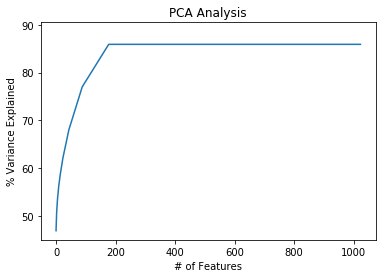
\includegraphics[width=0.4\textwidth]{images/componentAnalysis.png}
  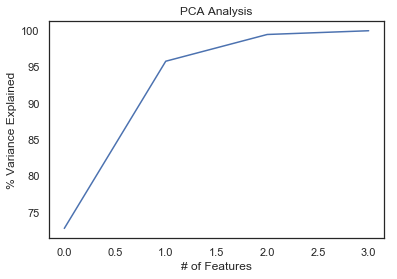
\includegraphics[width=0.4\textwidth]{images/irisComponentAnalysis.png}
  \caption{Component Analysis for PCA on PCam (left); Iris (right)}
\end{figure}

\begin{figure}
  \centering
  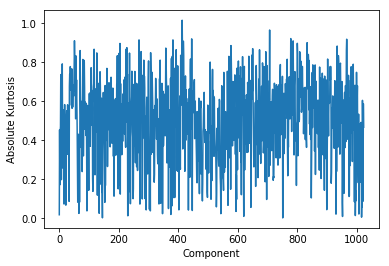
\includegraphics[width=0.4\textwidth]{images/pcaKurtosis.png}
  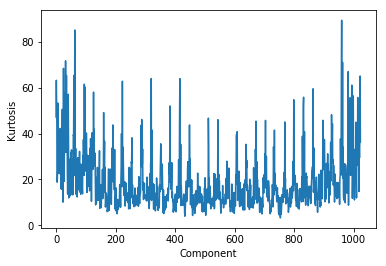
\includegraphics[width=0.4\textwidth]{images/icaKurtosis.png}
  \caption{Kurtosis for PCA's components (left); ICA's components (right) on PCam}
\end{figure}

\begin{figure}
  \centering
  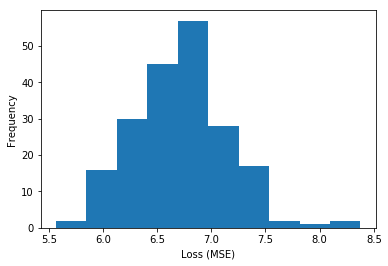
\includegraphics[width=0.4\textwidth]{images/randomDistr.png}
  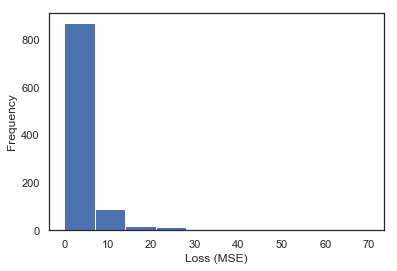
\includegraphics[width=0.4\textwidth]{images/randomDistrIris.png}
  \caption{Distributions for RP's MSE. PCam: 200 restarts, (left); Iris (right).}
\end{figure}


\begin{figure}
  \centering
  \begin{minipage}{0.45\textwidth}
    \centering
    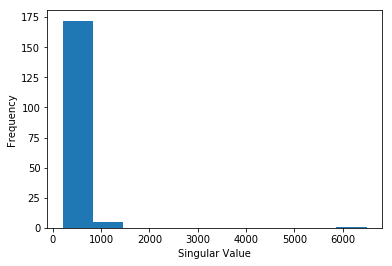
\includegraphics[width=0.9\textwidth]{images/singularDistr.png}
    \caption{Distribution for PCA's Singular Values (PCam).}
  \end{minipage}\hfill
  \begin{minipage}{0.45\textwidth}
    \centering
    \begin{tabular}{|l|l|}
      \hline
      \multicolumn{1}{|c|}{Singular Values} & \begin{tabular}[c]{@{}l@{}}20.89551896 \\ 11.75513248  \\ 4.7013819   \\ 1.75816839\end{tabular} \\ \hline
      Component Kurtosis Post-PCA & \begin{tabular}[c]{@{}l@{}}-0.67075488\\ -1.069148\end{tabular} \\ \hline
      Component Kurtosis Post-ICA & \begin{tabular}[c]{@{}l@{}}-0.67674155 \\ -1.08174288\end{tabular} \\ \hline
    \end{tabular}
    \caption{Singular Value and Kurtosis table for Iris}
  \end{minipage}
\end{figure}

\begin{figure}

\end{figure}

\section{Part II: Dimensionality Reduction}
In this subsection, I picked 178 components for PCA by looking at variance explained by number of components (Fig 9). I use the same number of components for ICA and RP to control this experiment.

\textbf{Note on picking components for ICA and RP:} The number of components chosen here are empirically arbitrary. In the case of PCA, we can directly analyze variance accounted for by the components. With ICA, our objective isn't to reduce the space -- instead, it's to find independent components; therefore each component in ICA is \underline{equally} important! PCA, however, has each component's importance weighed by its singular value (Fig 12, PCam or Fig 13, Iris).

For RP, I'll use the same number of components as PCA for control to see how much better/worse RP does with the same space constraint. Finally, the same methodology in subsection 2.1 was used to pick the optimal K for clustering on the dimensionality reduced dataset. Optimal values and metric scores can be seen in Table 1.

\subsection{Overview}
PCA works by finding orthogonal components that account for the most variance in a distribution. Each component is a linear combination of the underlying variables in this distribution. 

ICA works by finding components that transform the feature space so that it is independent. It also maximizes the information gain between the original feature space and the transformed space instead of maximizing variance as seen in PCA. To do this, ICA finds components that are as "non-gaussian" as possible/have high kurtosis. It turns out that these "non-gaussian" components are the key behind this reconstruction. An excellent argument for this line of reasoning can be found in Hyvärinen and Oja, 2000\autocite{Hyvarinen:2000:ICA:351654.351659}.

RP (Random Projections) are the simplest. We randomly pick a basis to project our dataset onto, and empirically evaluate the projections. Figure 11, left, shows the distributions of my projections of PCam, with 200 restarts. Note how the distribution matches the normal model (and follows CLT) because of the randomness. Therefore, it appears that it is quite hard to find a model with low loss. In the case of Iris (Figure 11, right) it is much easier to chance upon a low loss; however, note that we have a much larger number of restarts (1000) due to the smaller dataset size.

MSE Loss and Evaluation times for both PCam and Iris can be found in Table 2 and Table 3. Iris' dataset is too small to see significant change in evaluation time between each algorithm, except for the autoencoder. RP would also be faster if I used less restarts (there is a tradeoff).

Note the common bias: PCA and ICA work when the variance/independence can be explained linearly. Here's where the final dimensionality reduction algorithm comes in -- the autoencoder. 

\subsubsection{PCam Autoencoder}
I wanted to test a dimensionality reduction algorithm that worked on inherently non-linear data (most images). The autoencoder I used is of custom design; it is similar to the first half of the CNN used in Assignment 1, but symmetric. The output layer matches the input layer and I extract the middle layer as my encoders output. To maintain control in this experiment, the middle encoded layer has the same number of components as ICA and PCA (178).

\subsubsection{Iris Autoencoder}
For Iris, my autoencoder was just 2 dense layers with a ReLU activation function (adding non-linearity), with the encoded layer of dimension (2, 1). Figure 6 highlights the visualized projections.

\subsection{Extended Analysis}
To see if ICA actually finds these "non-gaussian" vectors, I plotted kurtosis values on PCA and ICA's components. In the case of PCam, Figure 10 highlights that ICA's absolute kurtosis is markedly higher than PCA's, as expected. However, Iris' PCA and ICA components (Figure 13) have similar Kurtosis, which sheds insight on why the ICA projection looks like a reflection of PCA. Perhaps the independent components happen to be the ones that explain variance.

Before I ran this experiment, I also hypothesized that PCA wouldn't perform as well as our non-linear dimensionality reduction algorithm, the autoencoder. Surprisingly, it performs quite well (Table 2 MSE reconstruction losses). I suspect that the non-linear assumption doesn't really hold for PCam as the images aren't representative of a picture someone would normally take.\footnote{Of all the images ever taken, how many are tumor tissue? Probably very few.} Therefore, the variance can be explained linearly.

ICA's relative reconstruction success also reinforces this suspicion since both PCA and ICA assume linear explainability, and both perform better than the autoencoder.

Because we can visualize Iris' projections, let's take a moment to look at them (projections with ground truth labelings in Fig 6). PCA and ICA look similar, except that the projections are reflected. Oddly enough, it looks like random projections result in the cleanest separations between different class labelings. RP also has the lowest MSE loss, as seen in Table 3. From these ground truth projections, we can hypothesize how well each algorithm might perform, and which algorithm we should use for clustering. This will be revisited in section 4.2.

\section{Part III: Dimensionality Reduction $\rightarrow$ Clustering}
As in Part I, we're using purity and V-Measure to define the good-ness of each cluster. The elbow method again dictates what value of K we decide to use.

\subsection{PCam}
For GMM, PCA performs better than the untouched dataset, and better than all other dimensionality reduction algorithms when the optimal value of K is chosen. This makes sense, as many samples of tumor tissue look similar aside from a few characteristics. Because of this, PCA can "remove" common features while maximizing variance to make clusters more separable. In the case of images, the gaussian distributions that performed relatively well are able to match the clusters better, increasing our overall performance. 

ICA performs noticeably worse on GMMs, perhaps because the independent components ICA finds aren't as useful as the variance. Furthermore, we only kept the most important components for PCA using feature analysis, and limited ICA to the same number (178) of components. For PCA, some components are more important than others (based on the magnitude of the singular values, see Fig 10); with ICA, all components are equally important. Because of this, we may be throwing out key components in ICA that account for the difference in accuracy.

The surprising outcomes are the Autoencoder and Random Projections. I expected the high MSE error for the Random Projections to carry over to low accuracy rates -- however, for some values of K (K=4), the random projections matched the untouched dataset. This makes me suspect that reconstruction error (MSE loss) may not be the best heuristic in determining the final performance of our clustering algorithm. The best explanation I can come up with is that some distinguishing feature is exaggerated when randomly projecting our dataset.

Our autoencoder performs the worst according to the V-Measure and Purity scores for the GMM. My suspicion is that the feature count limit that I used from PCA/ICA isn't enough to capture the non-linear features of our dataset. Because PCA does remarkably well compared to the autoencoder, I'm inclined to say that the autoencoder fails to follow Occam's razor. It attempts to fit a complex, non-linear model on a dataset than can be explained linearly -- and then fits poorly.

For KMeans, \textbf{3 algorithms perform exactly the same: PCA, random projections, and the untouched dataset.} I initially suspected that the cluster centers were, geometrically, exactly the same for PCA and the autoencoder. However, the high dimensionality of the untouched centroid disproves that -- geometrically, the clusters occupy different subspaces. My next hypothesis, which seems more likely, is that the hard clustering penalizes K-means for the same aforementioned reasons (section 2.2.1). Despite reducing the dimensionality of the original dataset, a static measure of distance won't distinguish the labels for key examples. The three algorithms are saving space and maintaining the original datasets structure, but they are not separating examples (between K-means' hard margins) in a way that benefits the clustering algorithm.

ICA suffers the most. I suspect that independent components do not work well with images and a distance metric. But the exact reason behind why it performs so much worse is unclear. I suspect that the ICA reconstruction affects the geometric structure of the dataset in a way that penalizes K-means (perhaps the samples become homogenous, something GMM can pick out).

Finally, the autoencoder begins to perform well as cluster sizes increase (the purity score especially), but the V-Measure stops increasing. Therefore, we aren't improving our ability to distinguish characteristics in the dataset, which furthers my hypothesis that PCam is better explained linearly.

\begin{figure}
  \centering
  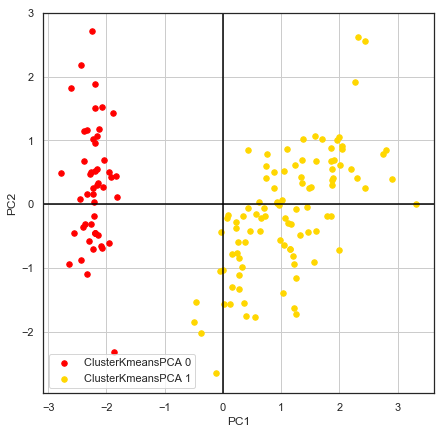
\includegraphics[width=0.4\textwidth]{images/curiousKmeansPCA.png}
  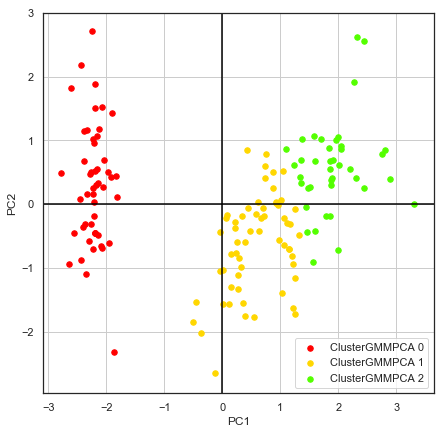
\includegraphics[width=0.4\textwidth]{images/curiousGMMPCA.png}
  \caption{Clustering on PCA Projected Dataset for KMeans (left); GMM (right).}
\end{figure}

\subsection{Iris}
Before dimensionality reduction, we saw that GMM performed far better than K-means. However, after running K-means and GMM on the projected PCA/ICA datasets, our metrics for the GMM drop to the same level as K-means (see table 1). 

Curiously, using 2 clusters for K-means on PCA reduced data actually results in a better V-measure than using 3-clusters. This suggests that getting an entire category incorrect provides more insight than splitting species up. Figure 14 (left) shows this preferred K-means clustering. For GMM on the PCA reduced data, our clusters aren't as hard as the K-means clusters, but it appears like GMM is more hesitant when compared to the clustering run on the original data (which is better than the PCA one). For reference, look at Figure 14 (right) and Figure 5 (right). Because the ICA and PCA projections are so similar, this might suggest the similar (bad) results.

Here is where RP shines: because our projected data's ground truth visually looks well separated (Figure 6, 4th), we know K-means will perform well (and it does!). Surprisingly, it does better than the unprojected dataset. This also holds for GMM, which does better than K-means and even better than the unprojected dataset.

This might actually highlight a drawback with our chosen metric, V-measure; it thinks that the insight gained by dropping a third cluster isn't valuable, yet our domain knowledge tells us it is.

Finally, our autoencoder performs the worst. Iris isn't inherently non-linear, so this might be another result of Occam's Razor (as with PCam).

\subsection{Note on Speed}
In the case of Iris, the speed difference between using a dimensionality reduced and non-reduced dataset isn't significant (Figure 8); however, this difference is visible with PCam (Figure 4).

\begin{table}
  \centering
  \begin{tabular}{l|c|c|c|c|c|c|c|}
  \cline{2-8}
  \multicolumn{1}{c|}{} & \multicolumn{1}{l|}{Original} & \multicolumn{1}{l|}{PCA} & \multicolumn{1}{l|}{ICA} & \multicolumn{1}{l|}{RP} & \multicolumn{1}{l|}{Autoencoder} & \multicolumn{1}{l|}{K-Means} & \multicolumn{1}{l|}{GMM} \\ \hline
  \multicolumn{1}{|l|}{$\mu$ Accuracy} & \textbf{.991} & .731 & .737 & \textbf{.897} & .722 & .751 & \textbf{.958} \\ \hline
  \multicolumn{1}{|l|}{$\mu$ Time} & 2.91 & 2.54 & 2.65 & 2.47 & 2.76 & 2.99 & 3.12 \\ \hline
  \end{tabular}
  \caption{$\mu$ Neural Network Classification Accuracy and Time after Dimensionality Reduction on 30 Trials}
  Section 6 describes how GMM and KMeans are used as Dimensionality Reduction Algorithms
\end{table}

\section{Neural Network Experiments \textcolor{red}{(Iris only)}}
\subsection{Overview}
The network used for Iris has 3 hidden layers (all ReLU, 10, 8, and 6 nodes in each dense layer) and one output layer (softmax, 3 nodes). The loss function used is categorical cross entropy. I used the Adam optimizer with a learning rate of .04. For the sake of control, none of the parameters were changed except for the size of the input layer. This is because some dimensionality reduction algorithms yielded different input sizes.

For the following subsections, I analyzed the average results of 30 trials on the Neural Network (Table 4) since the variance in results when using one trial was high -- this helped improve network performance for some algorithms. The original column in Table 4 summarizes results that come from a procedure used in Assignment 1. In other words, it's simply the accuracy and time of running the original dataset on the neural network learner.

Before I begin, here is a general procedure I used for assessing each network. If any change was made to the procedure, it is addressed in the following subsections.

\begin{enumerate}
  \item First, I withheld 10\% of the data-set, after shuffling, for final testing; the remaining 90\% fell into testing. I saved the random state to reproduce the splits.
  \item I ran the dimensionality reduction algorithms on both the train and test sets. Each reduction algorithm was fit on the entire dataset (train + test)
  \item Then, I trained the model on the test set, using optimal hyperparameter found using Assignment 1's procedures (cross validation on the test set, tune, retest, etc). 
  \item Finally, I would test on the withheld 10\% and take the average of 10 trials to reduce random variance. These are the results are in Table 4. 
\end{enumerate}

Finally, note that the time differences in Table 4 were insignificant due to the small size of Iris.

\subsection{Part IV: Dimensionality Reduction $\rightarrow$ Neural Network}
Compared to Assignment 1, all of the pure dimensionality reduction algorithms (PCA, ICA, RP, Autoencoder) do worse. This doesn't come as a surprise since our dataset is quite simple, and any loss in features results in decreased accuracy (i.e all features are important). Because our dataset's small size, there is no noteworthy difference in evaluation time.

The best dimensionality reduction algorithm on the network learner is the same as the one found in Part 2 -- random projections. Our visual projections showed that RP had the cleanest separations between classes (subsection 4.2 and Figure 6, 4th), and therefore performed the best on Iris. Also, our reconstruction loss with RP was the lowest, so RP performing the best on our network shouldn't come a surprise. This again highlights why RP appears to work so well in practice, given a sufficient number of restarts.
\subsection{Part V: Clustering $\rightarrow$ Neural Network}
To use clustering as our Dimensionality Reduction algorithm, I picked the optimal values of K (k=2 for K-means, 3 for GMM as seen in Table 1) for our untouched dataset. For K-means, our new input would be the distance of a sample from the centroid. For GMM, the new input would be the probability of our sample falling into each gaussian component.

Surprisingly, K-means and GMM serve as better dimensionality reduction algorithms then PCA and ICA when evaluated using a neural network. K-means, PCA, and ICA performing similarly makes sense -- all rely on linear assumptions. GMMs, however, uses normal/gaussian models to cluster. Compared to Assignment 1, GMM does very well, with only a 4\% difference in accuracy.

Because natural phenomena follow the normal model, it's not crazy to assume that the Iris species is distributed normally, and that GMM would reduce it well. Also, since k=3 for the GMM, we're losing only one dimension compared to two for the rest of reduction algorithm, which could also explain its improved performance.

All of this points to why GMM, as a dimensionality reduction algorithm, performs the best.
\printbibliography

\end{document}